\documentclass{../../PublicResources/DocClass}

    \DocumentTitle{免费商用字体}
    \DocumentCreatedDate{2019/8/6}

    \LinkBlogPost{}
    \LinkPDFSource{}
    \LinkVideo{}

    \AuthorName{Mr. Kin}
    \AuthorEmail{im.misterkin@gmail.com}
    \AuthorBlog{https://mister-kin.github.io/}

\begin{document}
    \pagenumbering{Roman} % 大写罗马字母样式页码。
    \maketitle
    \addcontentsline{toc}{chapter}{封面}
    \frontmatter
    \phantomsection
\begin{center}
    {\bfseries\sffamily\Large 关于作者}
\end{center}
\addcontentsline{toc}{chapter}{关于作者}

\subsection*{\bfseries \sffamily 关于我}
\begin{wrapfigure}[3]{L}{60pt}
    \vspace*{-20pt}
    \centering
    
\includegraphics{kin-logo}
\end{wrapfigure}
\textbf{Mr. Kin},广东客家仁,程序猿,CG和游戏爱好者,一枚极客。翻译UP主,个人UP主。不定时在B站直播日常:码代码,码博客,翻译,做视频,做教程。 ($\vartheta$$\bullet$\_$\bullet$)$\vartheta$ \hyperlink{follow}{\emph{(点击关注我!)}}

\subsection*{\bfseries \sffamily 开源建设}

\noindent {\bfseries \sffamily 开源软件的中文化翻译}

\begin{itemize}
    \item \href{https://docs.krita.org/zh_CN/}{Krita手册}:2018.8.5 - \href{https://crowdin.com/profile}{2019.4.23}
    \item \href{https://docs.blender.org/manual/zh-hans/latest/}{Blender手册}:2019.7.20 - \href{https://www.blendercn.org/5812.html?tdsourcetag=s_pctim_aiomsg}{2019.9.4} - 至今(\href{https://developer.blender.org/p/Mr_Kin/}{翻译维护})
\end{itemize}

\subsection*{\bfseries \sffamily \hypertarget{contact}{联系方式}}
\vspace*{-1ex}
\noindent {\footnotesize \color{red} \em 注:联系时请注明身份,谢谢!}

\begin{itemize}
    \item QQ:\href{tencent://AddContact/?fromId=45&fromSubId=1&subcmd=all&uin=2312463626&website=www.oicqzone.com}{2312463626}\emph{\color{red}(点击号码加好友)}
    \item 邮箱:2312463626@qq.com ; im.misterkin@gmail.com
\end{itemize}

\subsection*{\bfseries \sffamily \hypertarget{follow}{关注渠道}}
\vspace*{-1ex}
\noindent {\footnotesize \color{red} \em 注:点击文字即可跳转关注!}
\vspace*{-2ex}

\begin{figure}[htbp]
    \centering
    
\includegraphics[scale=0.2]{WechatOfficialAccounts.png}
\end{figure}
\vspace*{-4ex}

\begin{figure}[htbp]
    \centering
    \begin{minipage}[t]{0.2\textwidth}
        \centering
        \caption*{\href{https://mister-kin.github.io}{博客 - Blog}}
        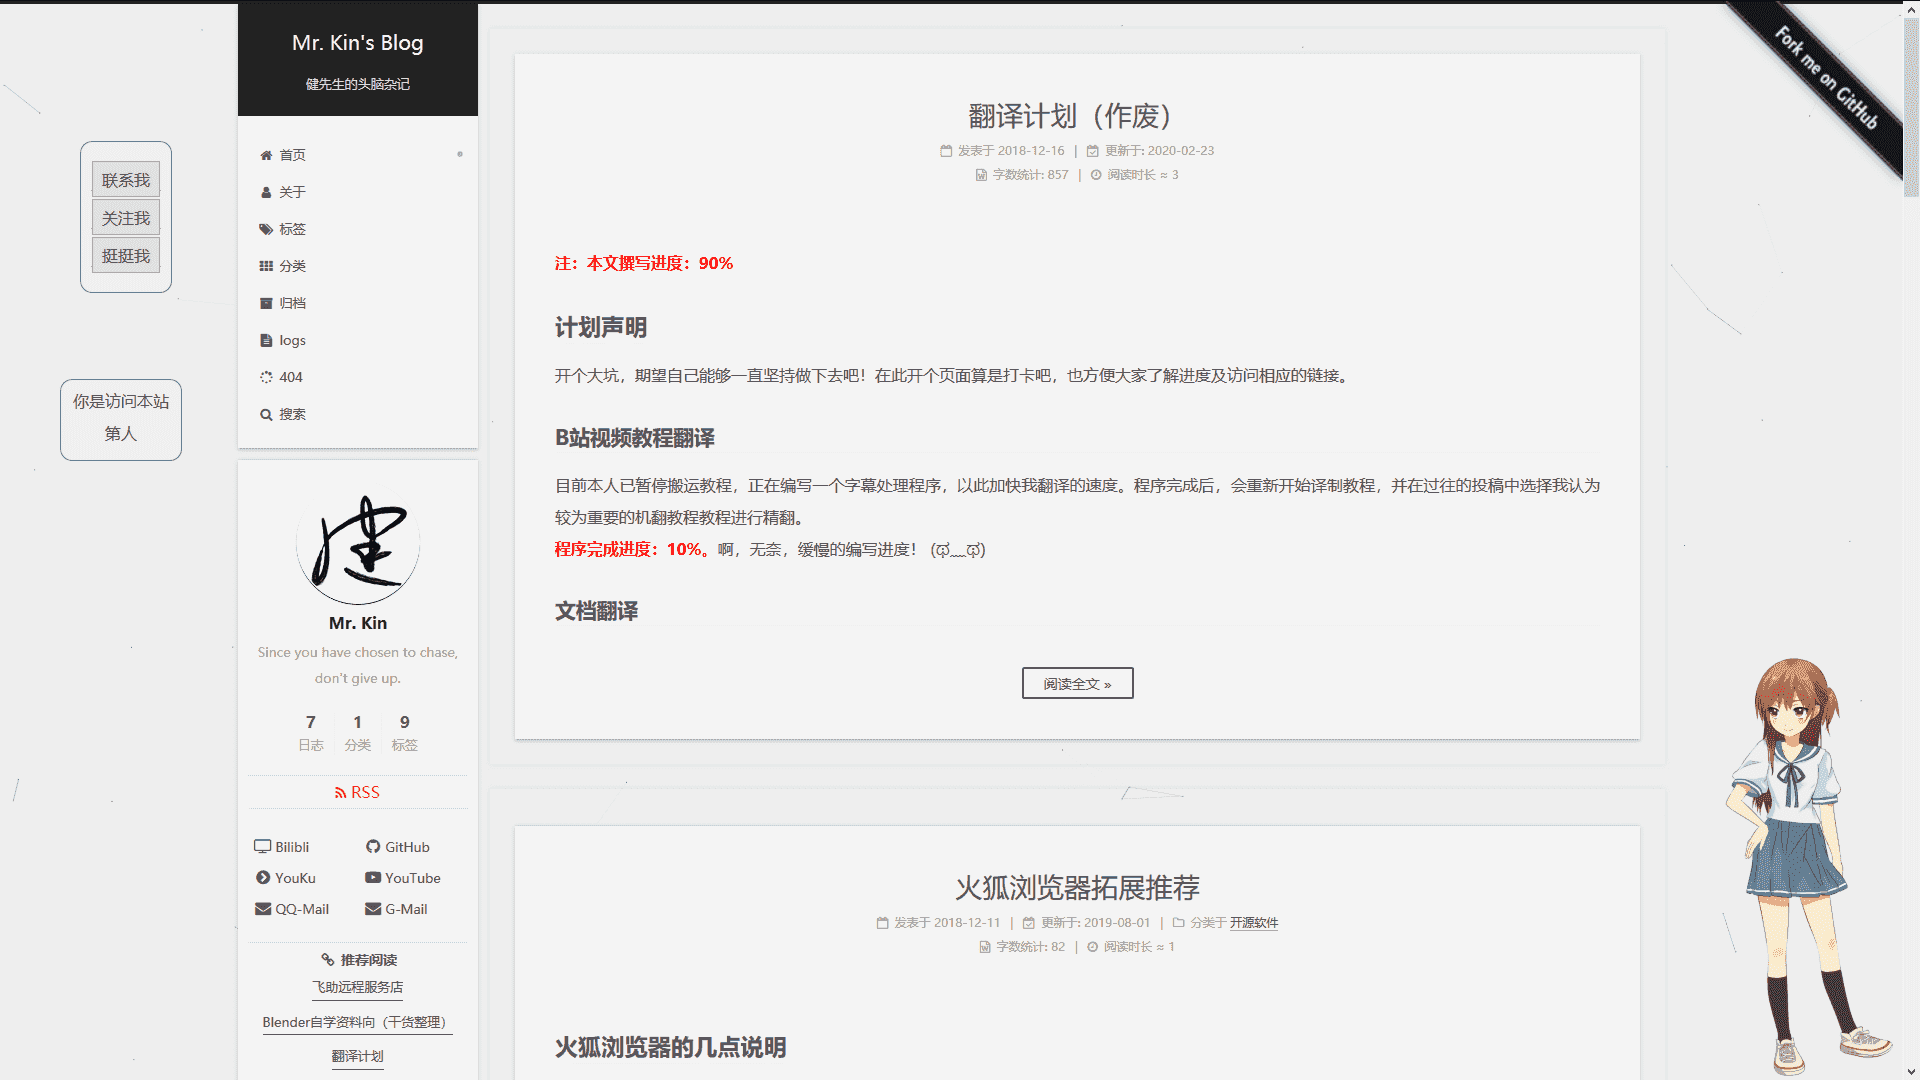
\includegraphics[scale=0.055]{Blog}
    \end{minipage}
    \qquad
    \begin{minipage}[t]{0.2\textwidth}
        \centering
        \caption*{\href{https://github.com/mister-kin}{Github}}
        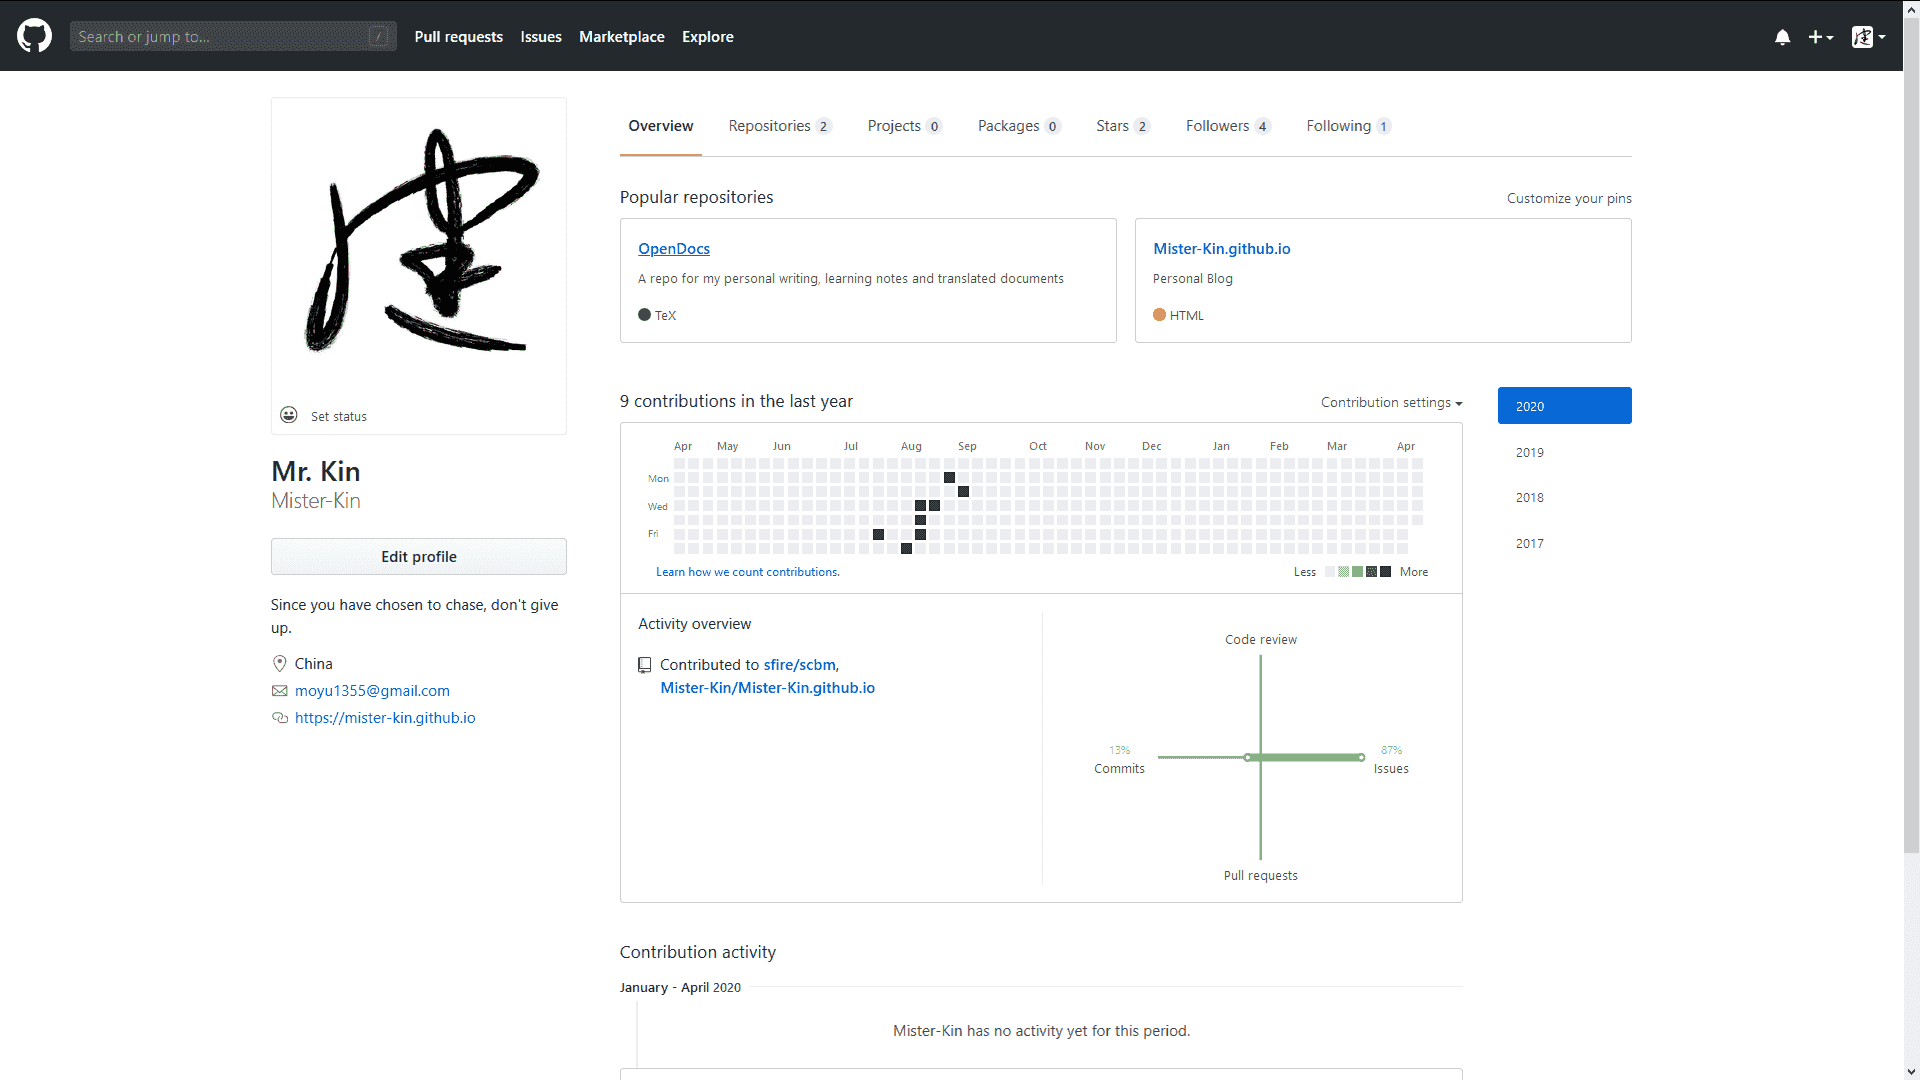
\includegraphics[scale=0.055]{Github}
    \end{minipage}
    \qquad
    \begin{minipage}[t]{0.2\textwidth}
        \centering
        \caption*{\href{https://weibo.com/6270111192/profile?topnav=1&wvr=6&is_all=1}{微博 - Weibo}}
        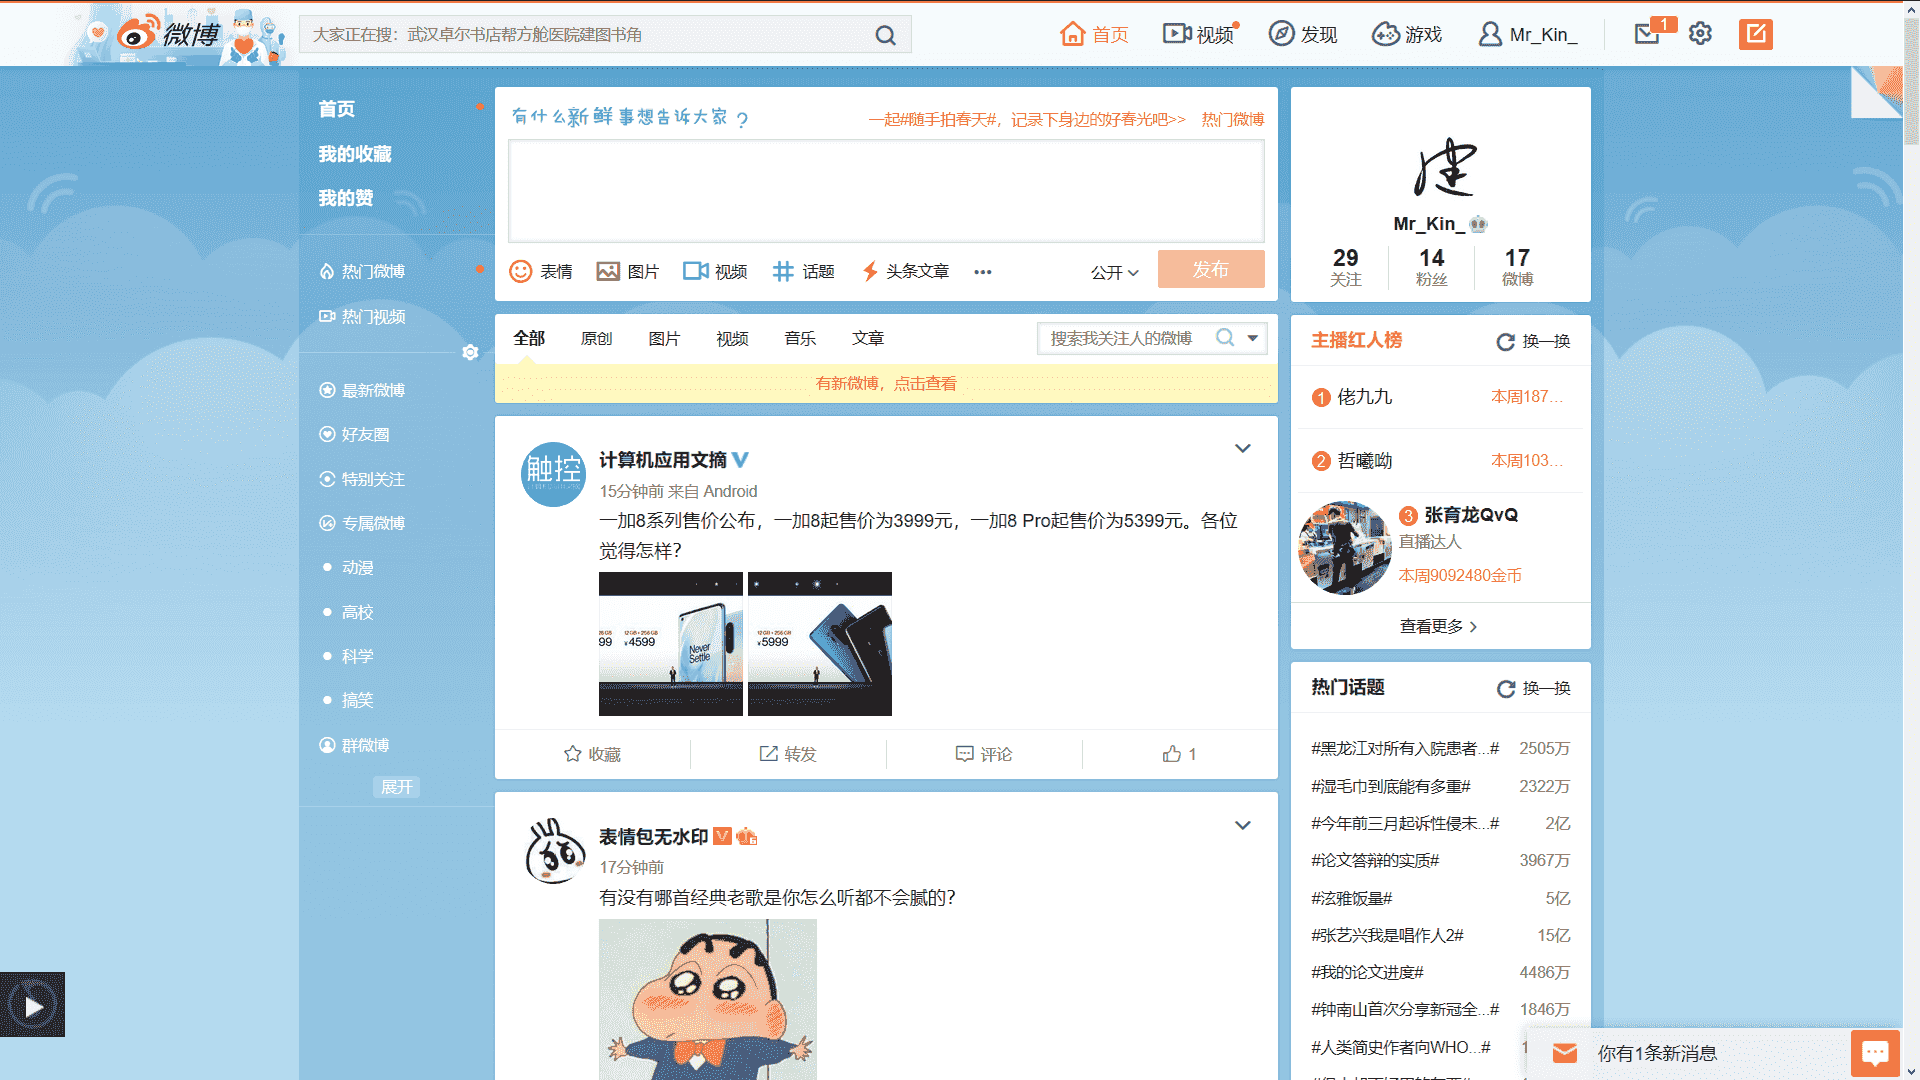
\includegraphics[scale=0.055]{Weibo}
    \end{minipage}
    \qquad
    \begin{minipage}[t]{0.2\textwidth}
        \centering
        \caption*{\href{https://www.zhihu.com/people/drwu-94}{知乎 - Zhihu}}
        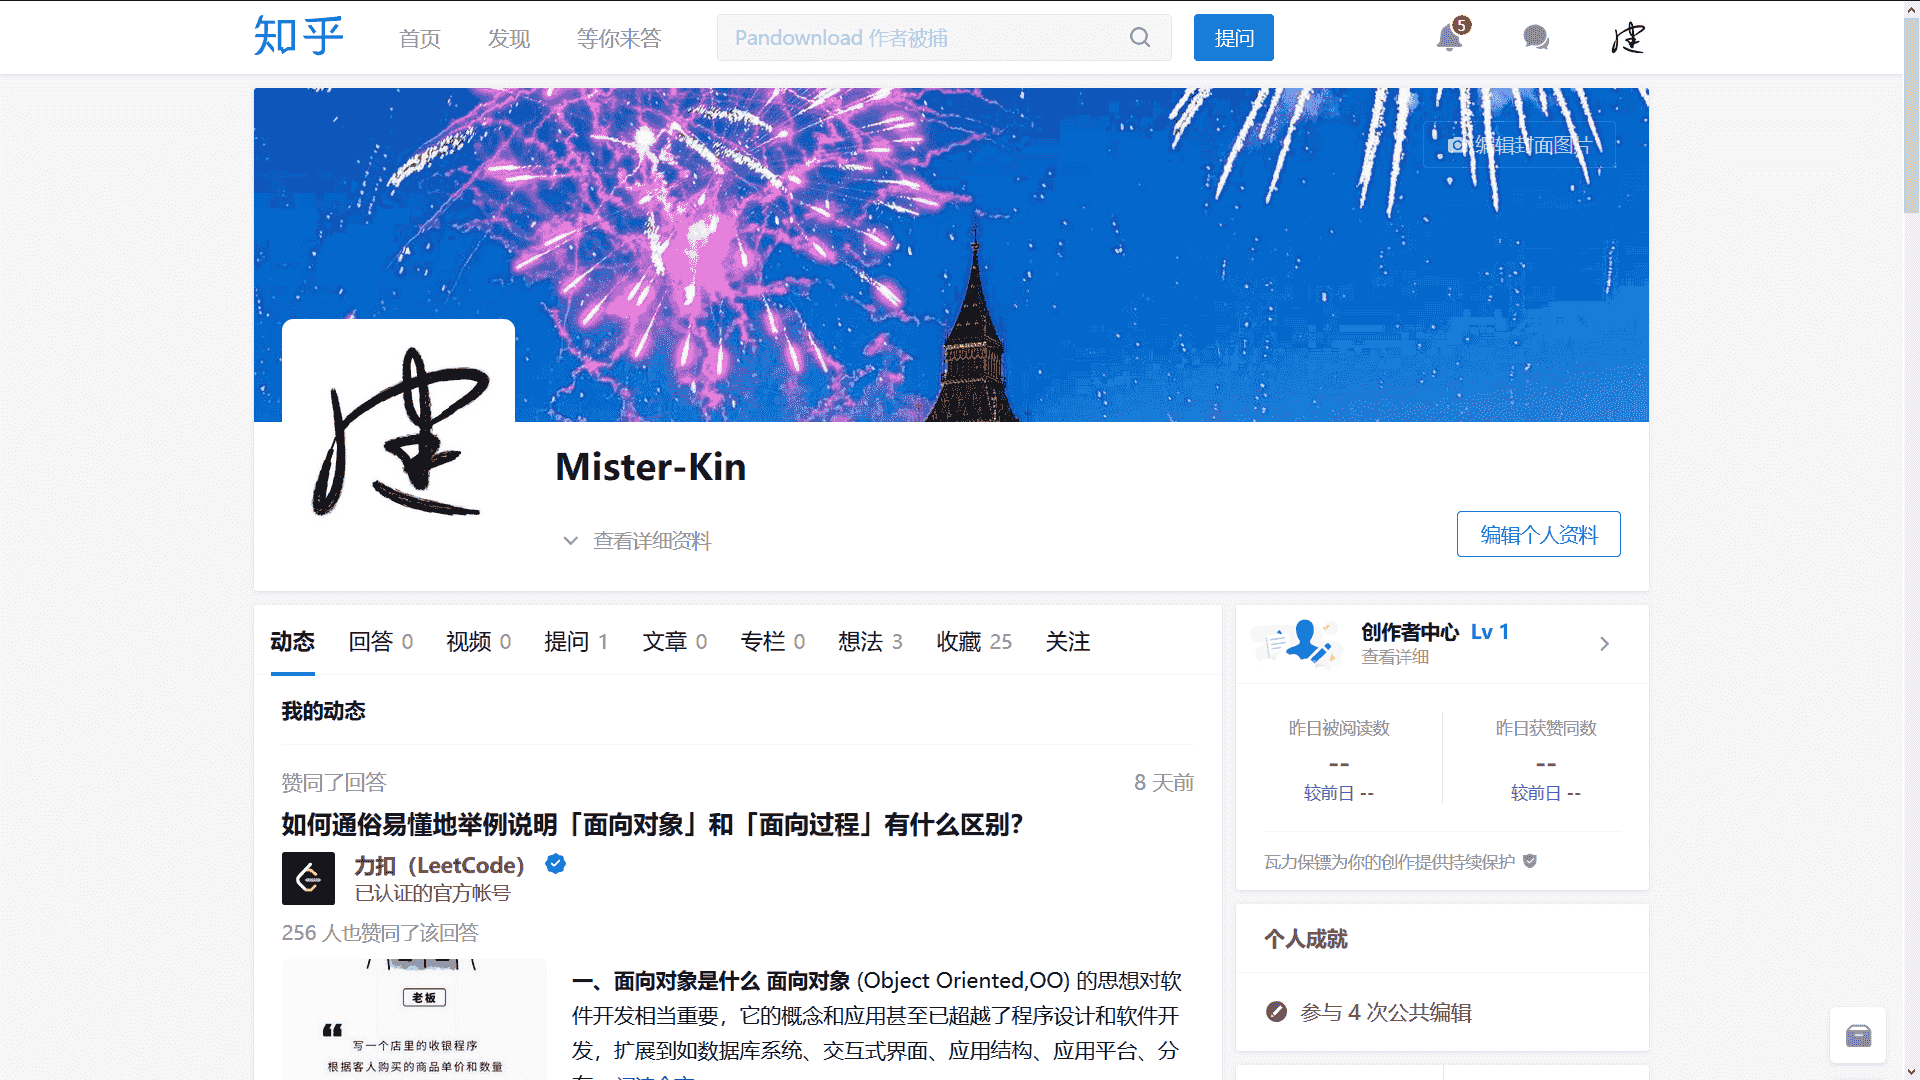
\includegraphics[scale=0.055]{Zhihu}
    \end{minipage}

    \vspace*{3ex}

    \begin{minipage}[t]{0.2\textwidth}
        \centering
        \caption*{\href{http://space.bilibili.com/17025250?}{B站 - Bilibili}}
        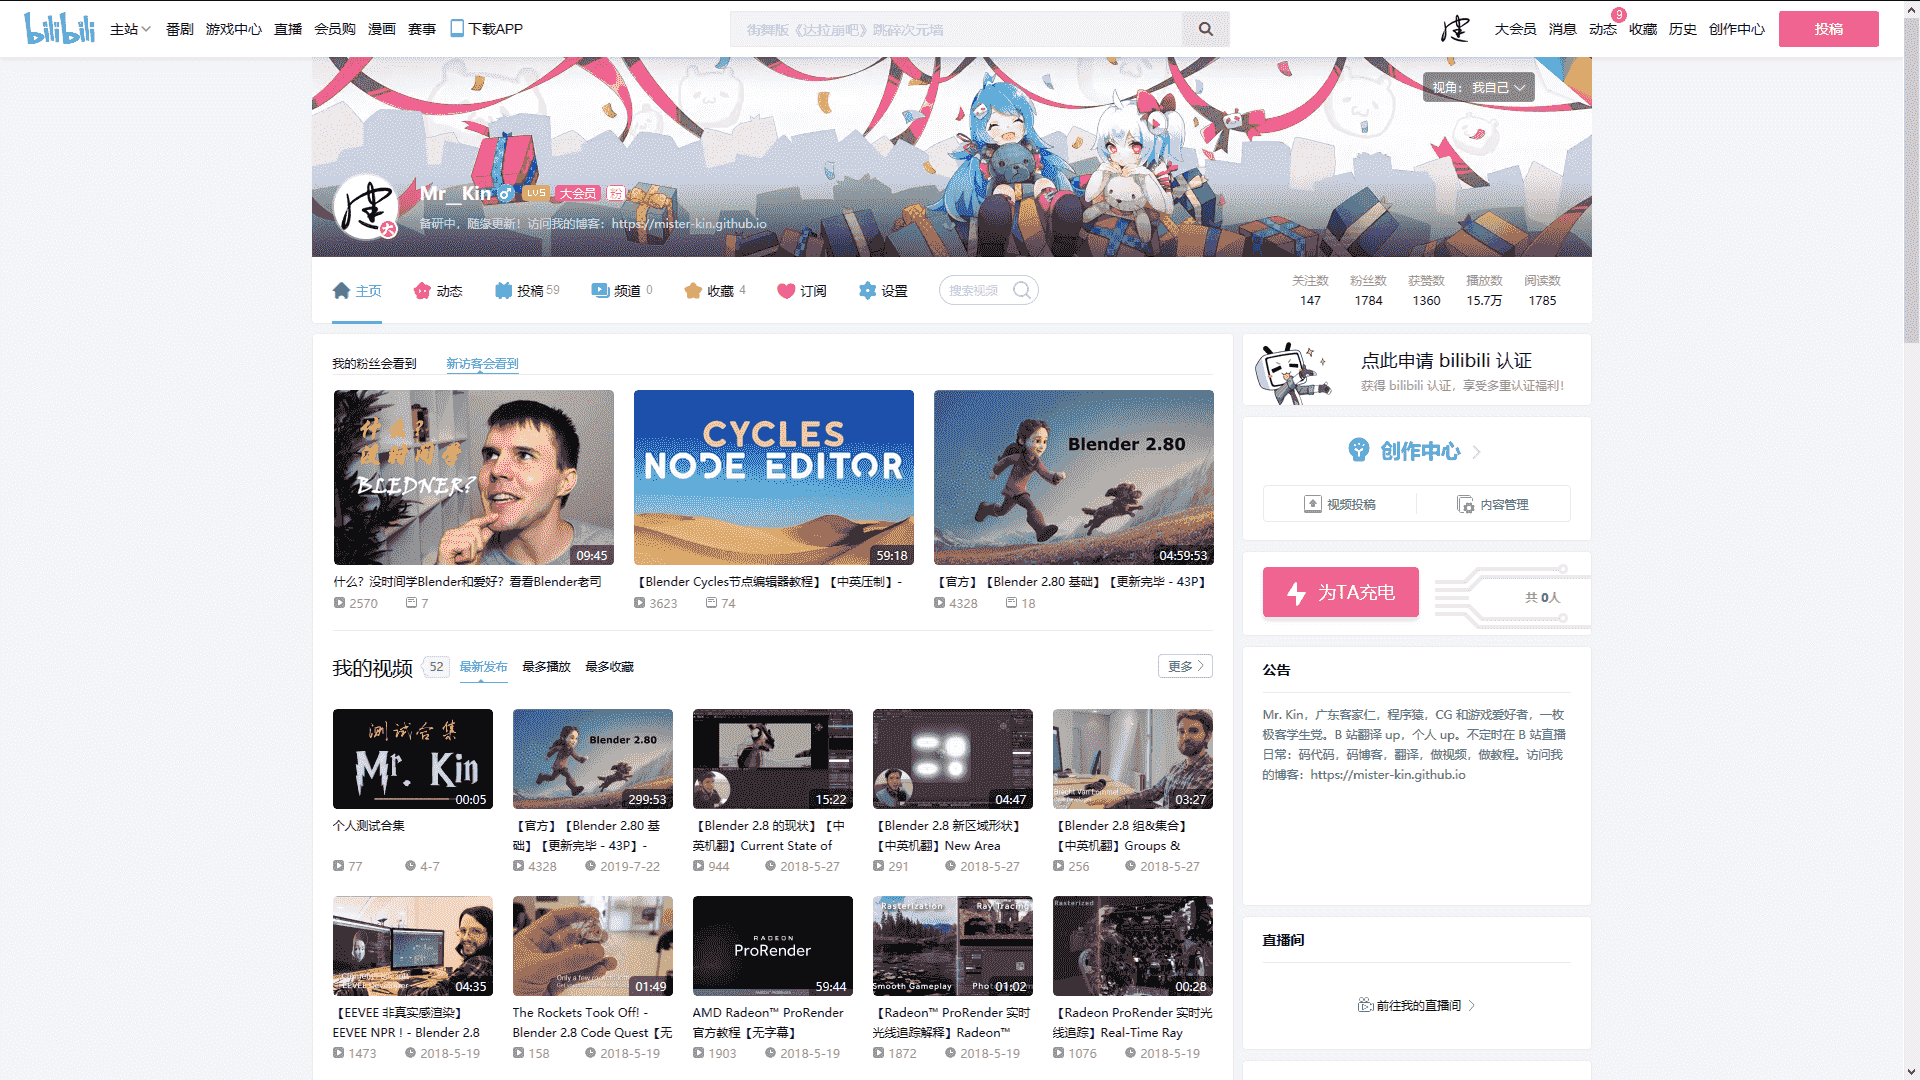
\includegraphics[scale=0.055]{Bilibili}
    \end{minipage}
    \qquad
    \begin{minipage}[t]{0.2\textwidth}
        \centering
        \caption*{\href{http://i.youku.com/i/UNjA3MTk5Mjgw?spm=a2hzp.8253869.0.0}{优酷 - Youku}}
        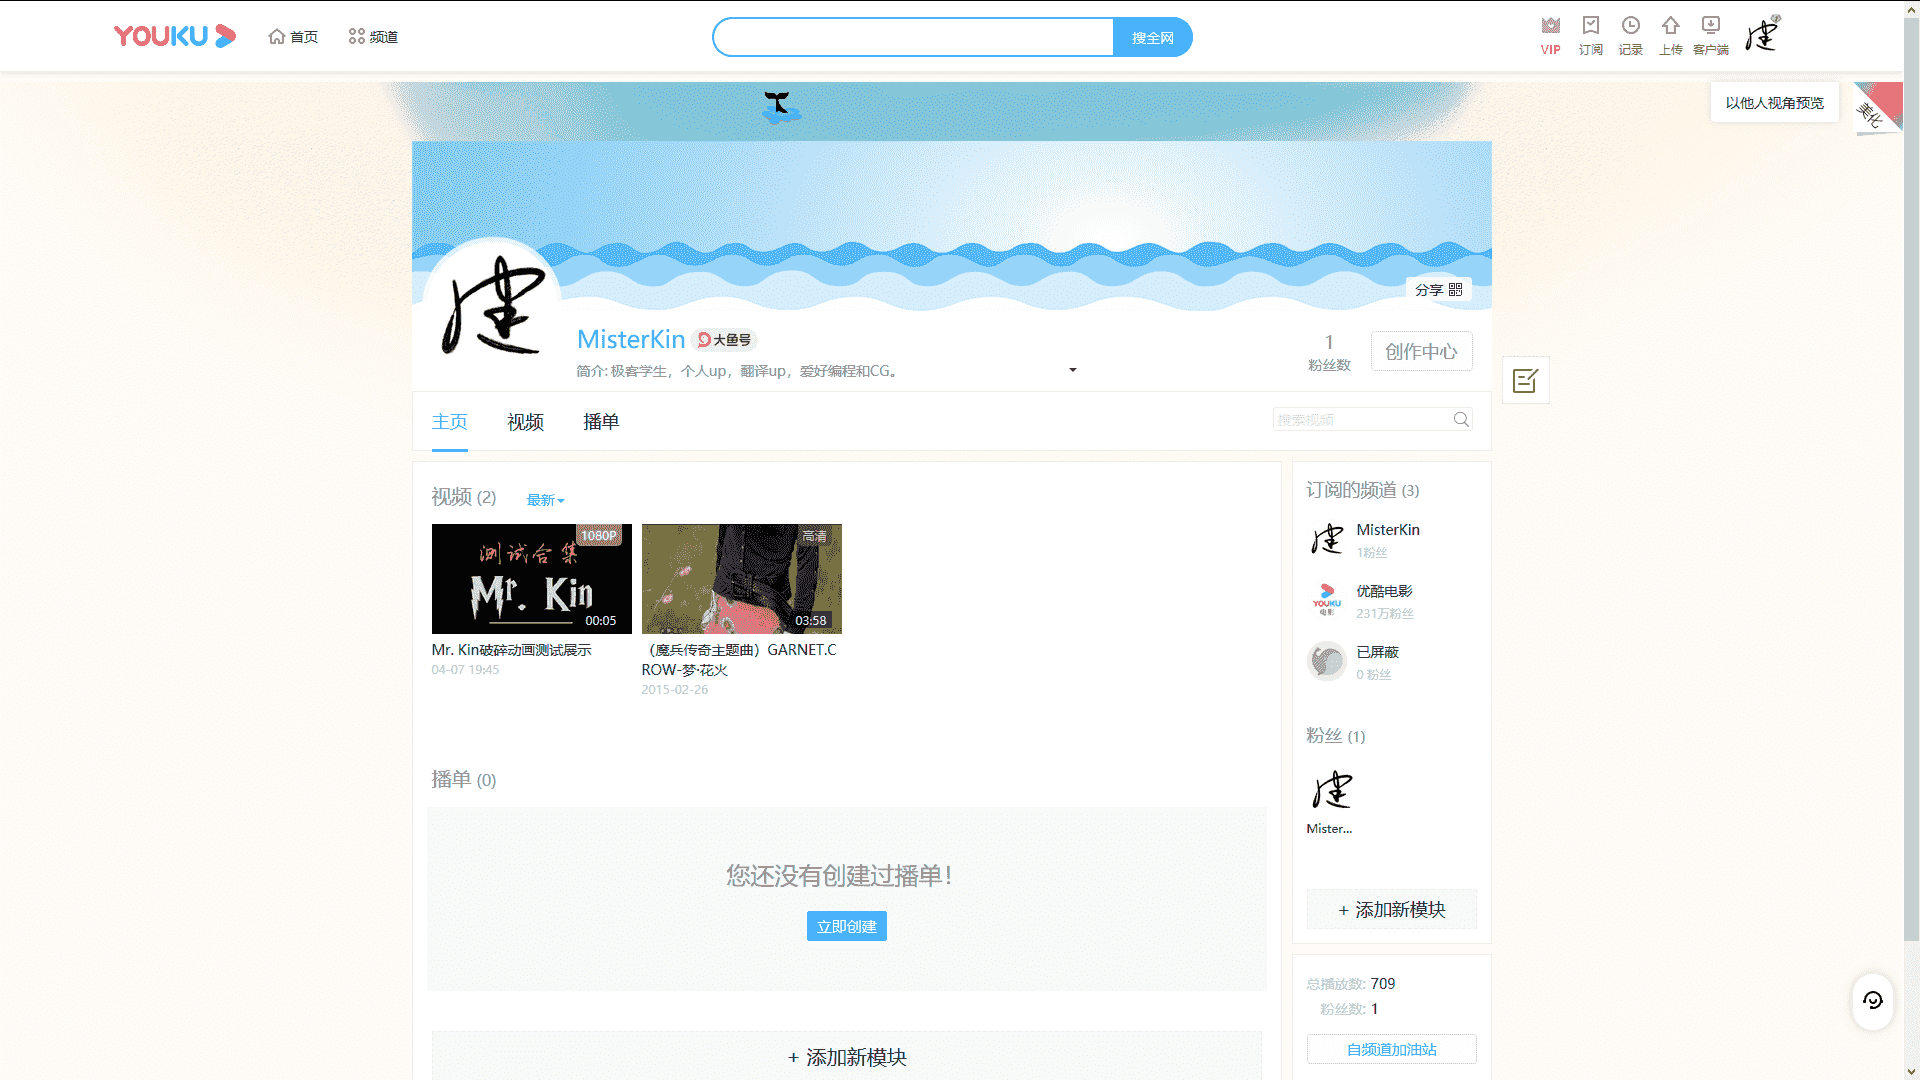
\includegraphics[scale=0.055]{Youku}
    \end{minipage}
    \qquad
    \begin{minipage}[t]{0.2\textwidth}
        \centering
        \caption*{\href{https://www.toutiao.com/c/user/835254071079053/\#mid=1663279303982091}{头条 - Headline}}
        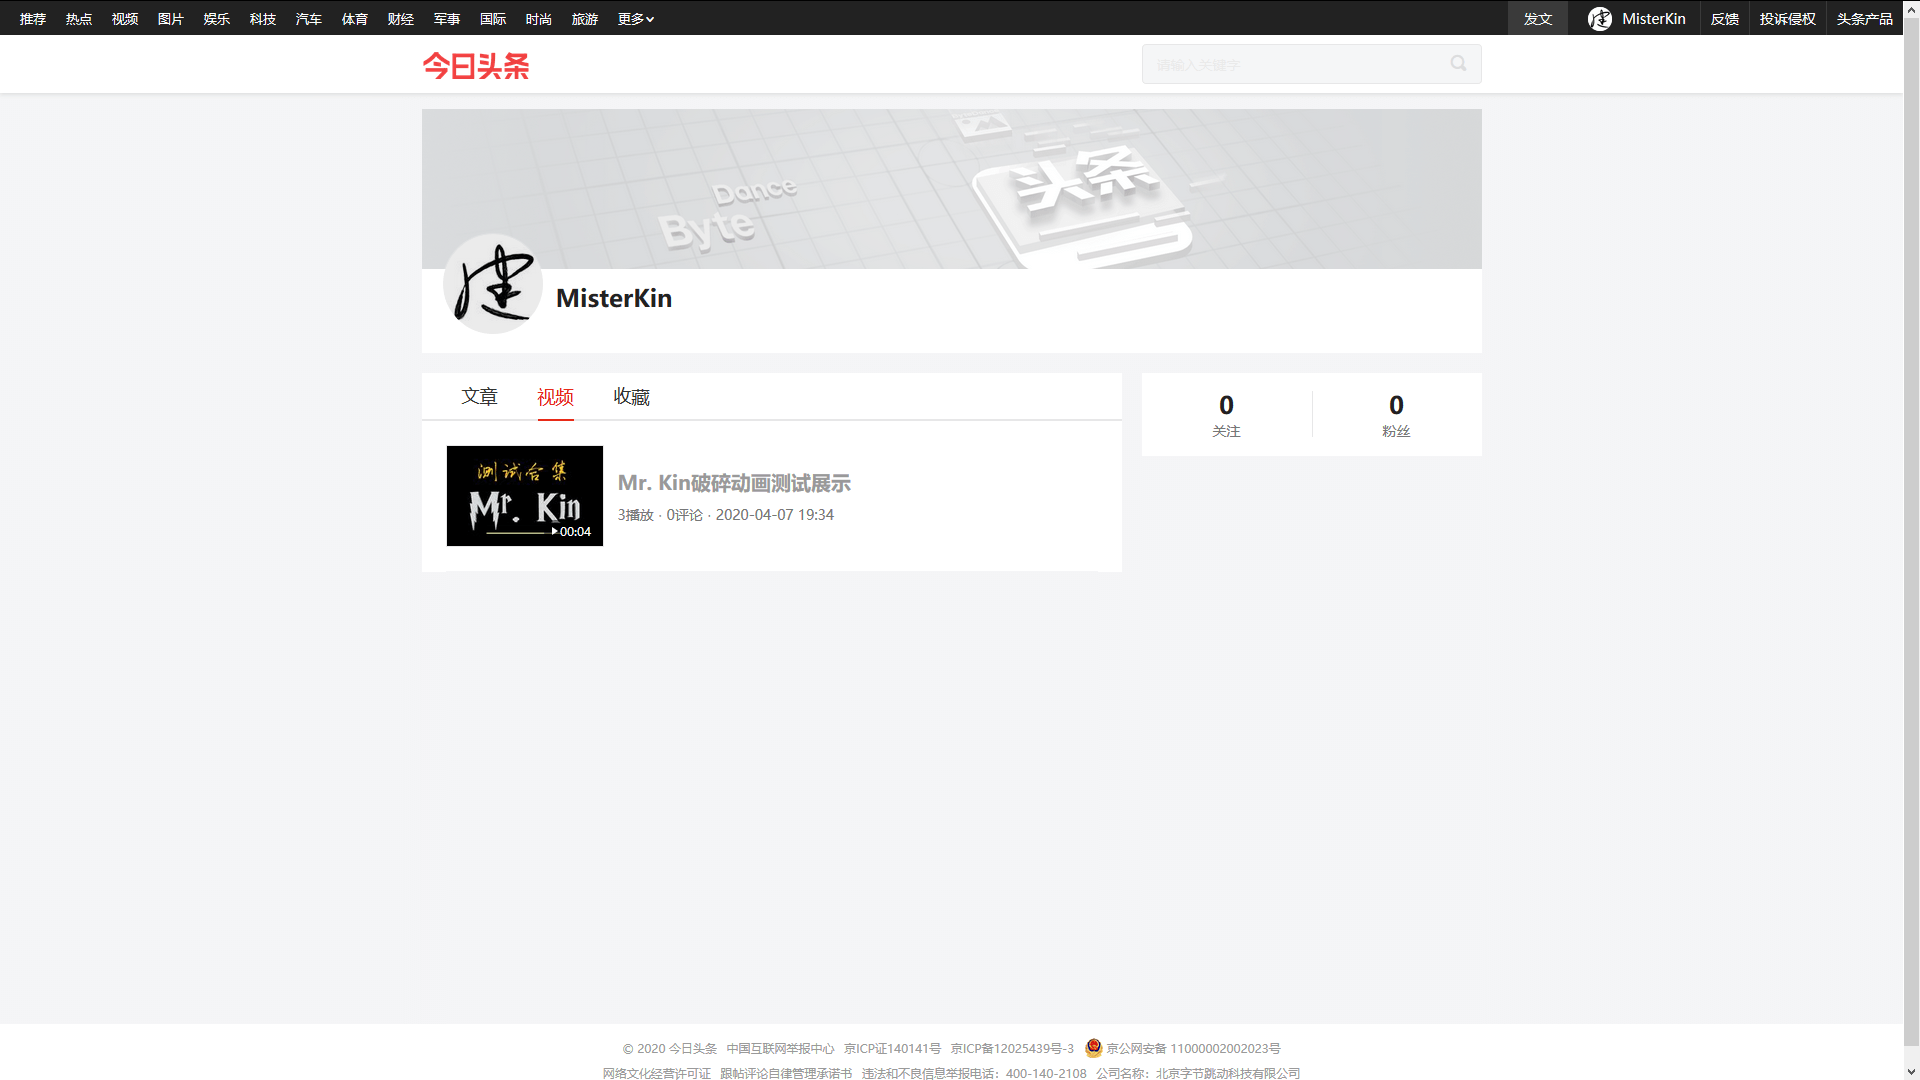
\includegraphics[scale=0.055]{Headline}
    \end{minipage}
    \qquad
    \begin{minipage}[t]{0.2\textwidth}
        \centering
        \caption*{\href{https://www.youtube.com/channel/UCXqjfWLzMlRKxGC8syWj17Q?view_as=public}{油管 - Youtube}}
        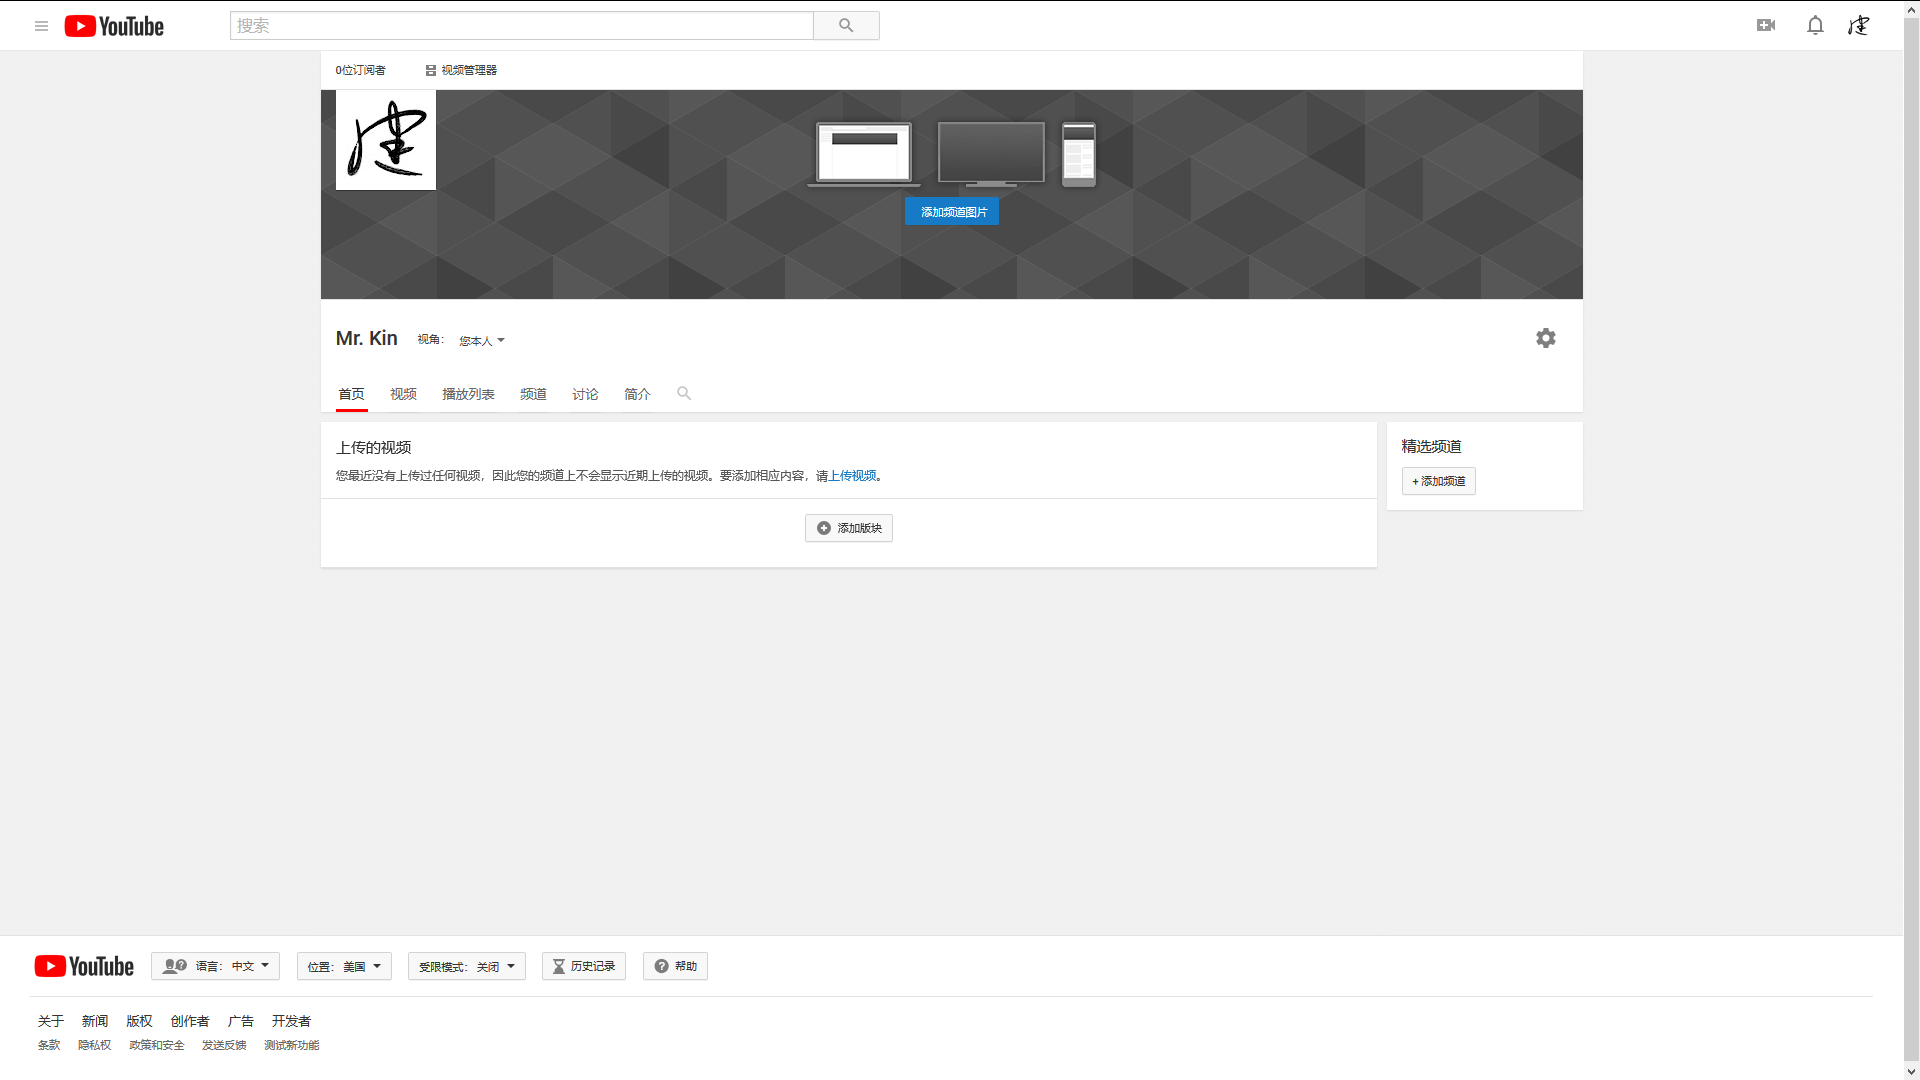
\includegraphics[scale=0.055]{Youtube}
    \end{minipage}
\end{figure}
 % 出于特殊的安全设置,\include 命令无法使用相对路径,因为需要读写权限以给 included file 写 aux 文件,而 \input 命令只需要读权限。
    \clearpage
    \phantomsection
\begin{center}
    {\bfseries\sffamily\Large 版权声明}
\end{center}
\addcontentsline{toc}{chapter}{版权声明}

\noindent 作者:Mr. Kin \\
\DetectToksEmpty\LinkBlogPost
\ifToksEmpty
博文链接:链接暂空\\
\else
博文链接:\href{\the\LinkBlogPost}{跳转博文页}\\
\fi
\DetectToksEmpty\LinkPDFSource
\ifToksEmpty
PDF及LaTex源码链接:链接暂空\\
\else
PDF及LaTex源码链接:\href{\the\LinkPDFSource}{跳转PDF及LaTex源码页}\\
\fi
\DetectToksEmpty\LinkVideo
\ifToksEmpty
\else
相关视频创作链接:\href{\the\LinkVideo}{跳转视频页}\\
\fi
许可协议:本作品的所有内容,除个人设计创作的图像(如logo等)和相关的视频创作及其他特别声明外,均采用\href{https://creativecommons.org/licenses/by-nc-sa/4.0/deed.zh}{知识共享\ 署名-非商业性使用-相同方式共享 4.0 国际许可协议}进行发布。版权 © Mr. Kin,保留所有权利。
\includegraphics[scale=.4]{CC-BY-NC-SA}\\*[1.3ex]
\begin{tabular}{|*{3}{p{0.306\textwidth}|}}
    \hline
    \textsf{\bfseries 允许} & \textsf{\bfseries 限制} & \textsf{\bfseries 条件} \\
    \hline
    \vspace{-8pt}{\color{green}√} 修改 & \vspace{-8pt}{\color{red}×} 商标使用 & \vspace{-8pt}{\color{blue}$\odot$} 保留原署名 \\[-12pt]
    {\color{green}√} 分发 & {\color{red}×} 专利使用 & {\color{blue}$\odot$} 状态变更说明 \\[-12pt]
    {\color{green}√} 个人使用 & {\color{red}×} 商业使用 & {\color{blue}$\odot$} 相同的许可和版权声明 \\
    \hline
\end{tabular}
\\*[1.3ex]
\emph{注:若想对本作品进行转载、引用亦或是进行二次创作时,请详细阅读上述相关协议内容(若不理解,请点击链接跳转阅读)。为保障本人权利,对于违反者,本人将依法予以处理!望周知!——Mr. Kin}

\begin{center}
    {\bfseries\sffamily\Large 勘误声明}
\end{center}

虽本人写作时已尽力保证其内容的正确性,但因个人知识面和经验的局限性以及计算机技术等相关技术日新月异,本作品内容或存在一些错误之处。还望诸君发现错误后能够\hyperlink{contact}{联系我}以更正错误,不胜感激!——Mr. Kin

\begin{center}
    {\bfseries\sffamily\Large 侵权声明}
\end{center}

若本作品采用的第三方内容侵犯了你的版权,请与我\hyperlink{contact}{联系}进行处理,谢谢!——Mr. Kin

\begin{center}
    {\bfseries\sffamily\Large 第三方开源许可声明}
\end{center}

\noindent 本作品使用的第三方开源产品有:
\begin{multicols}{2}
\begin{itemize}
    \item \href{https://github.com/adobe-fonts}{Adobe Fonts}: \href{https://github.com/adobe-fonts/source-serif-pro/blob/release/LICENSE.md}{OFL v1.1}
    \item \href{https://tug.org/texlive/}{Tex Live}: \href{https://tug.org/texlive/copying.html}{TeX Live Licensing}
    \item \href{https://code.visualstudio.com/}{Visual Studio Code}: \href{https://github.com/Microsoft/vscode/blob/master/LICENSE.txt}{MIT}
    \item \href{http://ffmpeg.org/}{FFmpeg}: \href{http://ffmpeg.org/legal.html}{LGPL v2.1 / GPL v2}
    \item \href{https://krita.org/en/}{Krita}: \href{https://docs.krita.org/en/KritaFAQ.html?highlight=license#license-rights-and-the-krita-foundation}{Krita's GPL license}
    \item \href{https://inkscape.org/}{Inkscape}: \href{https://inkscape.org/about/license/}{GPL}
    \item \href{https://www.gimp.org}{GIMP}: \href{https://www.gimp.org/about/COPYING}{GPL}
    \item \href{https://www.blender.org}{Blender}: \href{https://www.blender.org/about/license/}{GPL}
    \item \href{https://www.audacityteam.org/}{Audacity}: \href{https://www.audacityteam.org/about/license/}{GPL v2}
    \item \href{https://handbrake.fr}{Handbrake}: \href{https://github.com/HandBrake/HandBrake/blob/master/LICENSE}{GPL v2}
\end{itemize}
\end{multicols}

\noindent 更多请点击查看\href{https://mister-kin.github.io/about/third-party-declaration/}{第三方声明页}!

    \clearpage
    {\centering \tableofcontents} % 生成目录页。
    \mainmatter

    % 正文
    \chapter{安装方法}
    注:在win多用户平台上直接点击“安装”选项可能会使某些软件无法检测到该字体,例如Blender,故要“为所有用户安装”。部分软件不识别字体的中文名称,请找字族(Font Family)中对应的英文名称;若字族里无英文名称,那软件应该便会显示其中文名称。
    \section{单个字体安装}
    选择字体文件,右键点击选择“为所有用户安装”。
    \section{批量安装字体}
    选中多个字体文件(框选或者点击多选),右键点击选择“为所有用户安装”。

    \chapter{字体格式说明}
    \section{TTC}
    TTC字体是TrueType字体集成文件(.TTC文件),是在一单独文件结构中包含多种字体,以便更有效地共享轮廓数据,当多种字体共享同一笔画时,TTC技术可有效地减小字体文件的大小。TTC是几个TTF合成的字库,安装后字体列表中会看到两个以上的字体。两个字体中大部分字都一样时,可以将两种字体做成一个TTC文件,常见的TTC字体,因为共享笔划数据,所以大多这个集合中的字体区别只是字符宽度不一样,以便适应不同的版面排版要求。而TTF字体则只包含一种字型。

    \section{OTF}
    OpenType也叫Type 2字体,是由Microsoft和Adobe公司开发的另外一种字体格式。它也是一种轮廓字体,比TrueType更为强大,最明显的一个好处就是可以在把PostScript字体嵌入到TrueType的软件中。并且还支持多个平台,支持很大的字符集,还有版权保护。

    苹果机与PC机都能很好应用的兼容字体!

    \section{TTF}
    ttf版本的字体支持内嵌到Office文件,因此比otf技术底层的版本更适合与前端办公。

    PC机应用较好,苹果机兼容性很差!

    \chapter{开源字体集}
    开源不等于免费。GPL具有传染性,若GLP字体不附带「GPL 字型例外」(GPL font exception)协议进行阻断,则视为传染。因此,此列表一般不收集GPL字体。

    \noindent {\footnotesize \emph{注:字体打包中含有多格式时,如otf,ttf等,统一选择otf格式进行安装。}}

    \section{中文字体}
    如何使用繁体字:使用输入法输入繁体字,不要使用输入简体就可以得到繁体的字体。这类字体被称为“伪繁体”,在简繁转换上具有致命的缺陷。一些简体字与繁体字并不是一一对应的关系,而字体中编码和字形是一一对应的,所以伪繁体字库中这类简体字编码只能在多个对应的繁体字字形里选择一个来映射。使用伪繁体字库一般会出现这样的问题:输入人体部位 “头发”,得到的是错误的 “頭發” 而非正确的 “頭髮”。

    \begin{table}[h]
        \centering \caption{开源中文字体集}
        \begin{tabular}{|*{5}{c|}}
            \hline
            开发者 & 字体名称 & 英文名称 & 样式 & 授权协议 \\
            \hline
            \multirow{4}{*}{Adobe\&Google} & \href{https://github.com/adobe-fonts/source-han-sans/tree/release/}{思源黑体} & SourceHanSans & 简繁日韩|黑体 & \multirow{3}{*}{SIL OFL, v1.1} \\
            \cline{2-4}
            & \href{https://github.com/adobe-fonts/source-han-serif/tree/release/}{思源宋体} & SourceHanSerif & 简繁日韩|宋体 & \\
            \cline{2-4}
            & \href{https://github.com/adobe-fonts/source-han-mono}{思源等宽} & SourceHanMono & 简繁日韩|等宽 & \\
            \cline{2-5}
            & \multicolumn{4}{l|}{注:思源为Adobe版本的名称,google版本为NOTO(no toufo)} \\
            \hline
            \multirow{2}{*}{香港自由字型} & \href{https://freehkfonts.opensource.hk/download/}{自由香港楷书} & Free HK Kai 4700 & 繁|楷体 & CC-BY 4.0 \\
            \cline{2-5}
            & \multicolumn{4}{l|}{注:缺乏部分字型,如“国”字} \\
            \hline
            瀬戸のぞみ & \href{https://osdn.net/projects/setofont/}{瀨戸フォント} & setofont & 简繁日|艺术体 & SIL OFL, v1.1 \\
            \hline
        \end{tabular}
    \end{table}

    \clearpage
    \section{英文字体}
    \begin{table}[h]
        \centering \caption{开源英文字体集}
        \begin{tabular}{|*{4}{c|}}
            \hline
            开发者 & 字体名称 & 样式 & 授权协议 \\
            \hline
            \multirow{3}{*}{Adobe\&Google} & \href{https://github.com/adobe-fonts/source-sans-pro}{SourceSansPro} & 无衬线 & \multirow{3}{*}{SIL OFL, v1.1} \\
            \cline{2-3}
            & \href{https://github.com/adobe-fonts/source-serif-pro}{SourceSerifPro} & 衬线「罗马体」 & \\
            \cline{2-3}
            & \href{https://github.com/adobe-fonts/source-code-pro}{SourceCodePro} & 等宽「代码」 & \\
            \hline
        \end{tabular}
    \end{table}

    \chapter{免费商用字体集}
    \section{中文字体}
    \begin{table}[h]
    \centering \caption{免费商用中文字体集}
        \begin{tabular}{|*{5}{c|}}
            \hline
            开发者 & 字体名称 & 英文名称 & 样式 & 授权协议 \\
            \hline
            8:51:22 pm & \href{https://pm85122.onamae.jp/851fontpage.html}{851手書き雑フォント} & 851tegakizatsu & 简繁日韩|艺术体 & 可商用/修改分发 \\
            \hline
            林芳柽 & \href{https://www.zcool.com.cn/work/ZMjE0MjQyMDg=.html}{品如手写体} & 无 & 简|楷体 & 免费商用,禁转卖 \\
            \hline
        \end{tabular}
    \end{table}

    \section{英文字体}
    \begin{table}[h]
        \centering \caption{免费商用英文字体集}
        \begin{tabular}{|*{4}{c|}}
            \hline
            开发者 & 字体名称 & 样式 & 授权协议 \\
            \hline
            Phoenix Phonts & \href{https://www.fontspace.com/harry-p-font-f44342}{Harry P} & 艺术体「哈利波特」 & Freeware \\
            \hline
        \end{tabular}
    \end{table}

    \nocite{*} % 不使用 cite 也能生成参考文献。
    \printbibliography % 生成参考文献排版。
    \addcontentsline{toc}{chapter}{参考文献} % 添加参考文献进目录。

    \appendix
    % 附录
    \chapter{常见字体许可}
    \begin{enumerate}
        \item 商业字体:商业字体(Commercial)也就是正规的商业发行版,这种字体本应通过正规购买方式获得。

        \item 免费字体:免费字体(Freeware)是指用户可以无限制(包括:个人使用、商业使用)免费使用字体的版本,用户可能无法享用某些高级功能。其中有一部分免费字体通过自愿性的资助或者捐献,字体开发者从而获得补酬。

        \item 个人免费字体:个人免费字体是免费字体的子集,是指个人用户(不包括:商业使用)可以无限制免费使用字体的版本,用户可能无法享用某些高级功能。

        \item 共享字体:共享字体(Shareware)也包括试用字体(Trailware),是以“先使用后付费”的方式销售的享有版权的字体。根据共享字体作者的授权,用户可以从各种渠道免费得到它的拷贝,也可以自由传播它。用户可以先使用或试用共享字体,认为满意后再向作者付费;如果您认为它不值得您花钱购买商业授权,可以停止使用。

        \item 演示字体:演示字体(Demoware)是试用字体接近,但演示字体一般没有精减字形数量,但演示字体一般会在字形上打上特殊的标记或DEMO字样。

        \item 自由字体:自由字体(Free Software)向使用者提供没有任何限制的使用权限,遵循相关的自由软件授权协议允许任何人对该字体进行二次开发或用于商业用途,甚至有时会提供字体源代码,这种也称为开源字体(Open Source)。

    \end{enumerate}

    \chapter{方正字库“商业发布”授权价格说明}
    方正字库“商业发布”授权价格说明(2016年2月起正式施行)

    计算机字库是典型的拥有著作权的作品。根据中华人民共和国著作权法,使用他人作品应当同著作权人订立许可使用合同。著作权人 未明确许可、转让的权利,未经著作权人同意,另一方当事人不得行使。

    计算机字库的使用方式主要有以下三种:
    \begin{enumerate}
        \item 内部使用:指个人或单位在其内部使用的终端设备上安装并使用字库的行为。该使用行为包括在屏幕上显示和临时从打印机上输出两种。
        \item 内置使用:指将字库文件整体或部分、直接或格式转换后,以嵌入的方式应用到网站、计算机程序或带有可视化显示功能的电子产品中的行为。
        \item 商业发布:指以直接营利或者间接营利为目的,将字体作为视觉设计要素,进行复制、发行、展览、放映、信息网络传播、广播等使用字体的行为。
    \end{enumerate}

    据法律,任何使用方式都必须事先获得著作权人得授权。未经授权使用字体将面临侵权的风险。上述三种方式中 “商业发布”行为是字体应用最重要的一种方式。方正公司仅针对商业发布内容的最终所有者提供授权。 由于商业发布行为涉及的用户种类多,范围广,形式复杂。为了最大程度的满足最大多数用户最通常的使用,同时又能保障字体创作者的劳动价值,方正公司针对“商业发布”行为将方正字体分为“免费字体”、“基础字体”和“精选字体”三类:

    免费字体:包括四种字体:方正黑体、方正书宋、方正仿宋、方正楷体。针对“商业发布”这种使用方式免费。

\end{document}
